%-----------------------------------------------------------------
% Requirements and/or Problem Section(s):
% In this section you should describe the problem or system you are addressing in detail. Describe the project requirements and constraints.
%-----------------------------------------------------------------
\subsection{Design Problem}
The problem we are trying to solve is to beat daily fantasy basketball competitions using machine learning with neural networks. In order to fully understand this problem, it is important to detail the specifics of these daily fantasy basketball competitions. 
\subsubsection{Competition Choice}
Although fantasy competitions are often thought of as long-term league competitions with drafting and brackets, these were not the types of competitions that we targeted. There are many different types of competitions with varying rules. Instead of trying to create a system that can compete in all of these competitions, we decided to target a subset, which met a set of criteria:
\begin{itemize}
\item Daily fantasy competitions
\item Low entry fee (< \$10)
\item Allow for multiple entries
\item High prize pool and participant count
\end{itemize}
Daily refers to the fact that the competitions are on a given day where real basketball games are being played and involve only the games being played that day, with no residual effects on future competitions. Fantasy refers to the fact that the competitions use an arbitrary points system. Allowing multiple entries means that multiple lineups can be submitted to the same competition. A header for one of these competitions from FanDuel.com can be seen in figure \ref{fig:comp_header}. This header shows the low entry fee of \$7, the high prize pool of \$100,000, and that multiple entries are allowed. It also shows a list of the real games that are occurring that night.

\begin{figure}[ht]
    \centering
    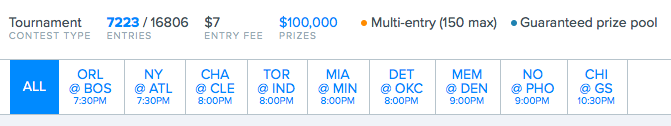
\includegraphics[width=0.75\textwidth]{figures/fantasy_competition_header}
    \caption{Daily NBA fantasy competition header}
    \label{fig:comp_header}
\end{figure}

One of the criteria of the Picking Winners paper was that the prize pool be "top-heavy". With top-heavy competitions, "contests give a disproportionately high fraction of the entry fees to the top scoring lineups." \cite{picking_winners}. The entry fees for these competitions are usually less than \$10, and the top placing competitors usually win thousands of dollars. The payout structure of a top-heavy competition with a \$4.44 entry fee and \$400,000 prize-pool can be seen in Figure \ref{fig:comp_payout}.

\begin{figure}[ht]
    \centering
    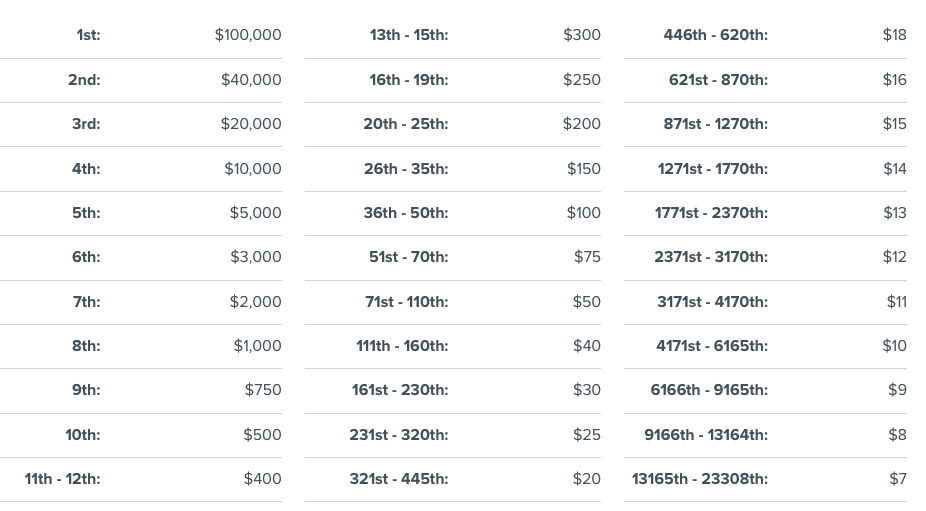
\includegraphics[width=0.75\textwidth]{figures/fantasy_competition_payout}
    \caption{FanDuel daily fantasy competition payout}
    \label{fig:comp_payout}
\end{figure}

One can see that the monetary difference between first and tenth place is 200 times, whereas the monetary difference between tenth and one-hundredth is only 10 times. The idea behind participating in a top-heavy competition is that, even if many of your lineups do not win, one or two may win a lot, offsetting the losses of the other entries. Hunter  et al. \cite{picking_winners} felt that some of their lineups could come in the top 10 of these competitions, and that they thus had a higher expected value participating in these top-heavy competitions. One reason we felt we also had a chance at a high ranking entry is that we believed that our system could return uncommon selections of players for our lineups that other methods (intuition or optimization) would not return. The reason that this could be beneficial is because, usually, less-picked players are cheaper, and thus a good but less-picked player would generate more points per dollar spent, allowing for a higher total score. However, we were not strict on this requirement, and participating in other types of contests, including 50-50 contests, where the top 50\% of competitors are given near double their entry fee.

\subsubsection{Entries}
After selecting the competition to enter, the participant must create an entry, or lineup. This lineup must comprise players that are playing in the real games on that day. Additionally, the lineup must have a certain amount of specific basketball positions. A common requirement is that the lineup must have two point guards (PG), two shooting guards (SG), two power forwards (PF), two small forwards (SF), and one center (C). Note that these positional requirements are not necessarily representative of a real basketball team. Figure \ref{fig:comp_lineup} shows the lineup selection interface for FanDuel.com. On the right side, one can see the required positions for a given competition, along with the lineup's budget, in the top right corner. This budget is the amount of money each contender is allowed to spend on their lineup. On the left side, one can see the price of each player, along with their position, and their average fantasy performance for the season, on which the price is dependent.

\begin{figure}[ht]
    \centering
    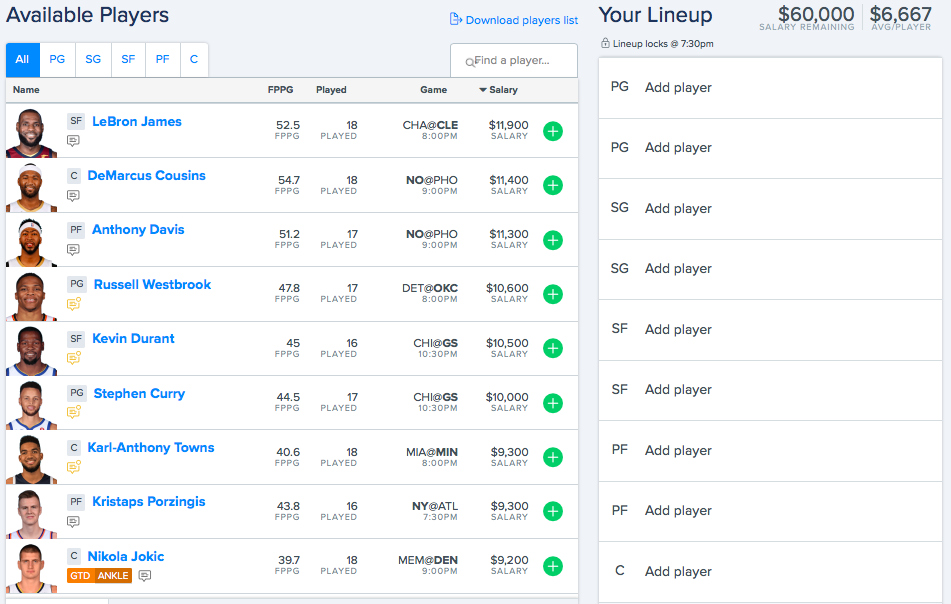
\includegraphics[width=0.75\textwidth]{figures/fantasy_competition_lineup}
    \caption{Fantasy basketball competition lineup}
    \label{fig:comp_lineup}
\end{figure}

\subsubsection{Scoring}
The participant's goal is to have the lineup with the highest score. The score is based on how well their selected players perform in real life, and is based on the amount of free throws, three pointers, field goals, blocks, steals, assists, and turnovers each player gets. The scoring system for competitions on FanDuel can be seen in Figure \ref{fig:comp_scoring}.

\begin{figure}[ht]
    \centering
    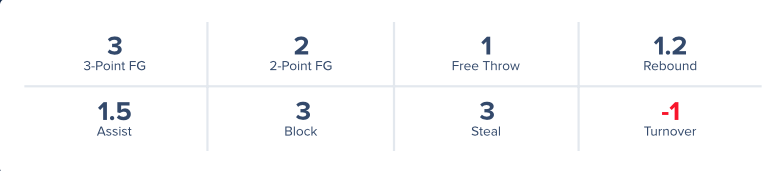
\includegraphics[width=0.75\textwidth]{figures/fantasy_competition_scoring}
    \caption{Fantasy basketball competition scoring}
    \label{fig:comp_scoring}
\end{figure}

\subsection{Requirements and Constraints}
In order to solve the described problem, we had to comply with the rules of the competitions mentioned above. However, we also had to abide by other requirements and constraints, detailed in this section.
\subsubsection{Functional Requirements}
%(e.g. what a product should do)
\begin{itemize}
\item The system should be able to use all previous NBA data
\item The system should be able to output lineups for daily fantasy competitions based on which teams are playing, how much each player costs, and which positions are needed
\item The system should output a projected score for each lineup
\end{itemize}

\subsubsection{Usability Requirements}
%(e.g. security, network, platform, integration, client)
\begin{itemize}
\item The system should use a MySQL database
\item The database should be secure and have personalized credentials for all users
\item The system source code should be version controlled
\end{itemize}

\subsubsection{Technical Requirements}
\begin{itemize}
\item The system should be able to train to convergence on the order of minutes, so as to allow for cross-validation on the order of hours (or at most, a couple of days)
\item The system should be modular, allowing for easy architectural alteration (e.g. changing a scoring algorithm)
\item The system should also allow the NN hyperparameters, such as the learning rate, amount of data used for training, and architecture, to be altered easily
\end{itemize}

\subsubsection{Constraints}
\begin{itemize}
\item The system should not require any expensive services
\item The system should be trainable on our personal computers (but not necessarily be able to be cross-validated on our computers)
\item The system must be completed within eight months (two university terms)
\end{itemize}